\documentclass[twoside,11pt]{article}

% Any additional packages needed should be included after jmlr2e.
% Note that jmlr2e.sty includes epsfig, amssymb, natbib and graphicx,
% and defines many common macros, such as 'proof' and 'example'.
%
% It also sets the bibliographystyle to plainnat; for more information on
% natbib citation styles, see the natbib documentation, a copy of which
% is archived at http://www.jmlr.org/format/natbib.pdf

\usepackage{jmlr2e}
%\usepackage{parskip}

% Definitions of handy macros can go here
\newcommand{\dataset}{{\cal D}}
\newcommand{\fracpartial}[2]{\frac{\partial #1}{\partial  #2}}
% Heading arguments are {volume}{year}{pages}{submitted}{published}{author-full-names}
 
% Short headings should be running head and authors last names
\ShortHeadings{95-845: MLHC Article}{Tripathi and G}
\firstpageno{1}

\begin{document}

\title{Heinz 95-845: Article Title on \\Machine Learning and Health Care}

\author{\name Tanmaya Tripathi \email ttripath@andrew.cmu.edu \\
       \addr Heinz College\\
       Carnegie Mellon University\\
       Pittsburgh, PA, United States
       \AND
       \name Xin G \email xing1@andrew.cmu.edu \\
       \addr Heinz College\\
       Carnegie Mellon University\\
       Pittsburgh, PA, United States} 

\maketitle

\begin{abstract}
 
 \textbf{Background -} The cases of abnormal urine flow rate have increased over the past few years. There has been significant changes in the lifestyle of the humans since the Information Age. The study aims to understand if there is any relationship between lifestyle choices such as nutrition and physical activity to a person's urine flow rate output.


\vspace{5mm}  \textbf{Methods - } To conduct the study we extracted the entire NHANES data set going back to the 1999-00 dataset. From this dataset we extracted patient demographics data, nutrition data, basic health data and bladder health data. After data cleansing we were left with 1981 patients. The patients were excluded due to conditions such as missing values. Furthermore, the study revolved around men aged 20-45 years old. Post cleansing statistical methods such as Logistic Regression were implemented to extract significant variables. To further augment the results, Machine Learning techniques such as Decision Trees and Random Forest were used.


\vspace{5mm} \textbf{Findings - } Out of all the variables accounted for the variable DEQ034D (Use of sunscreen) was highly significant with a p-value of approximately 0.004. The average accuracy of the models was 86\% with random forest giving the highest accuracy. However, if the test set was accounted for all the algorithms were performing at the same level.


\vspace{5mm} \textbf{Interpretation - } The study in its current format highlights that there is some kind of correlation between use of sunscreen and the urine flow rate. In fact as you decrease the use of sunscreen the chances of having a regular urine flow rate increase. However, the study needs to be further developed. Due to lack of data several columns were removed from the analysis. Hence, it is highly likely that there is an excluded variable which relates better to the outcome and also explains the relationship shown above.
\end{abstract}

\section{Introduction}

Since the dawn of time, mankind has slowly changed his/her lifestyle. Rather than being an outgoing, hunting and caveman type civilization we have now moved into brick and mortar homes, domesticated animals and grow our own crops. This change has been very predominant/accelerated since the 1950s, the start of Information Age. Therefore, it is clear that there have been significant changes in the way we humans live. However, it is yet unclear as to how such rapid changes affects one's health. The goal of this project is to understand this change and how to better adopt to it.

\vspace{5mm} Studies till date have shown that urinary hesitancy is caused by several factors such as stress, bacterial infection, cancer, excessive drinking etc. However, we are still unclear as to what are the social situations which lead to the outcome. Does a patient's income, geoghraphic region, type of job etc have any effect on whether the person will suffer from an abnormal or decreased urine flow rate.

\vspace{5mm} Our study aims to help understand what are the differences in the lifestyle between an individual with a healthy urine flow rate vs the opposite.


\section{Background} \label{background}


To conduct this study we used the NHANES (National Health and Nutrition Examination Survey) dataset. We extracted the data from 1999-00 to 2013-14. From the NHANES dataset we extracted Demographics data, Laborartory data and Quetionairre data. This data was then combined together to extract the useful rows. However, it is at this stage that we ran into an issue. The NHANES team started collecting data for Urine flow from the year 2009 onwards. Therefore, this greatly reduced our sample size since we had to omit all the rows before 2009. Going further we extracted the male population aged between 20 to 45 years. Hence, at the end of the extraction we were left with 1,981 rows out of which 1,740 patients had a regular flow rate while 241 patients had an abnormal flow rate.
\vspace{5mm} \textbf{The data extraction process flow diagram has been shown below-} figure ~\ref{fig:Extraction_Process_Flow}
\begin{figure}[htbp]
  \centering 
  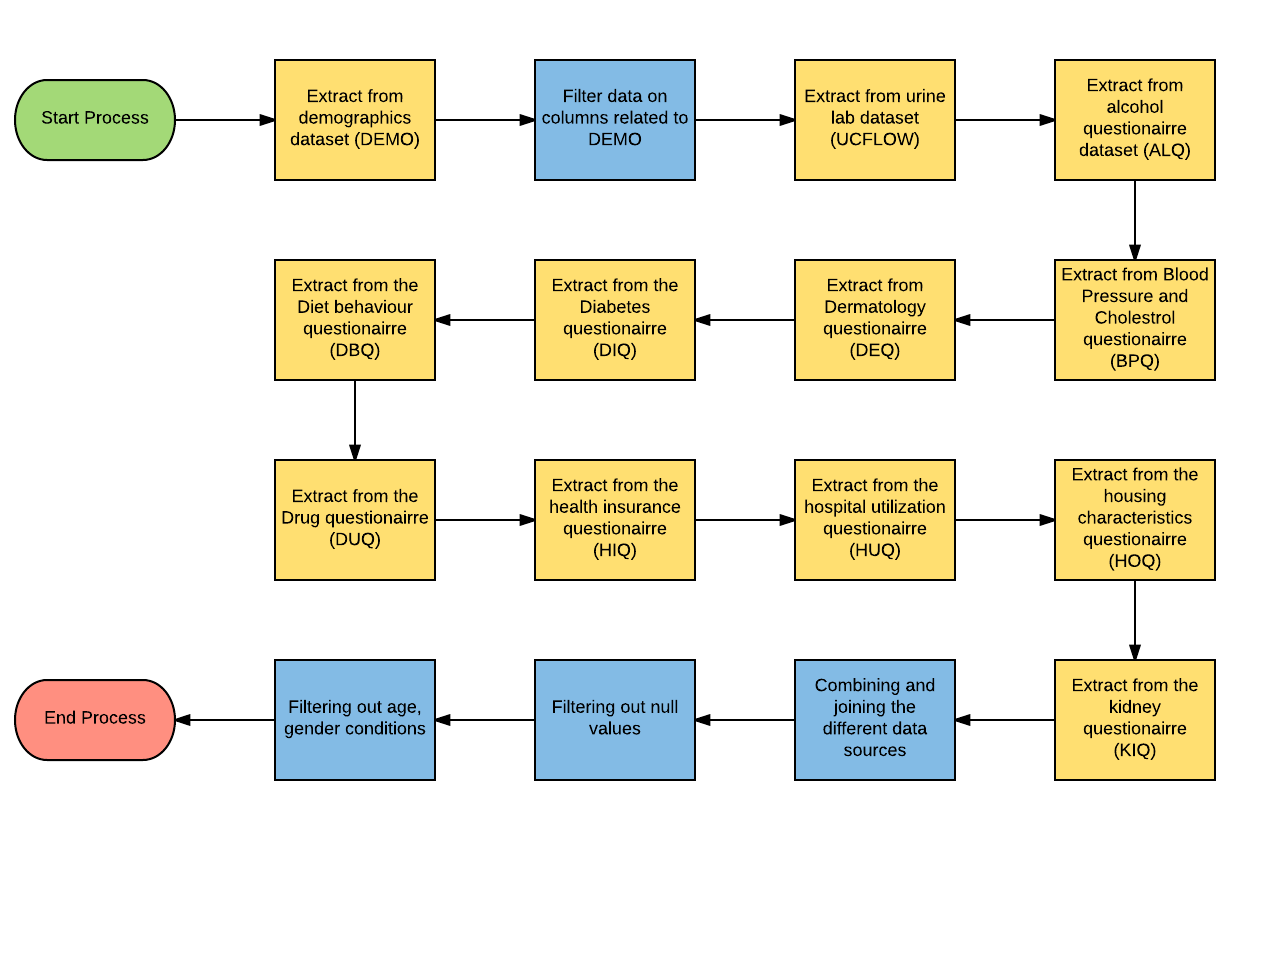
\includegraphics[width=4.5in]{data_extraction_process.png} 
  \caption{Extraction Process Flow.}
  \label{fig:Extraction_Process_Flow} 
\end{figure} 

\section{Methods} \label{methods}
To start with we used a basic Logistic Regression model. This was to understand the significane of the differene columns with respect to the outcome of the final column. The first step was to prepare the data for the model. For this we did the following operations-

\textbf{a.} Converted columns to factors or numerics as mandated.

\textbf{b.} Converted the factor columns to dummy columns. Therefore all factor based columns now have values 1 or 0.

\textbf{c.} Assigning Yes to value 1 and No to value 0.

\vspace{5mm} Post data preperation we developed the Logistic Regression model from the binomial family. Upon acquiring the summary of the model we found one column in particular significant. This was column DEQ034D. The column captures the patient's use of sunscreen and is part of the dermatology data set. The values of the column are shown in figure ~\ref{fig:Sunscreen_Data}
\begin{figure}[htbp]
  \centering 
  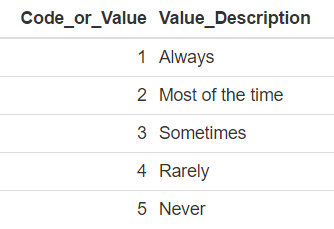
\includegraphics[width=2in]{sunscreen_data.png} 
  \caption{Sunscreen Data.}
  \label{fig:Sunscreen_Data} 
\end{figure} 

The p-value for the above column was approximately 0.004. To further understand this relation we developed a plot between the urine flow rate and the use of sunscreen. The graph in figure ~\ref{fig:Graph_SD} shows the relation.

\begin{figure}[htbp]
  \centering 
  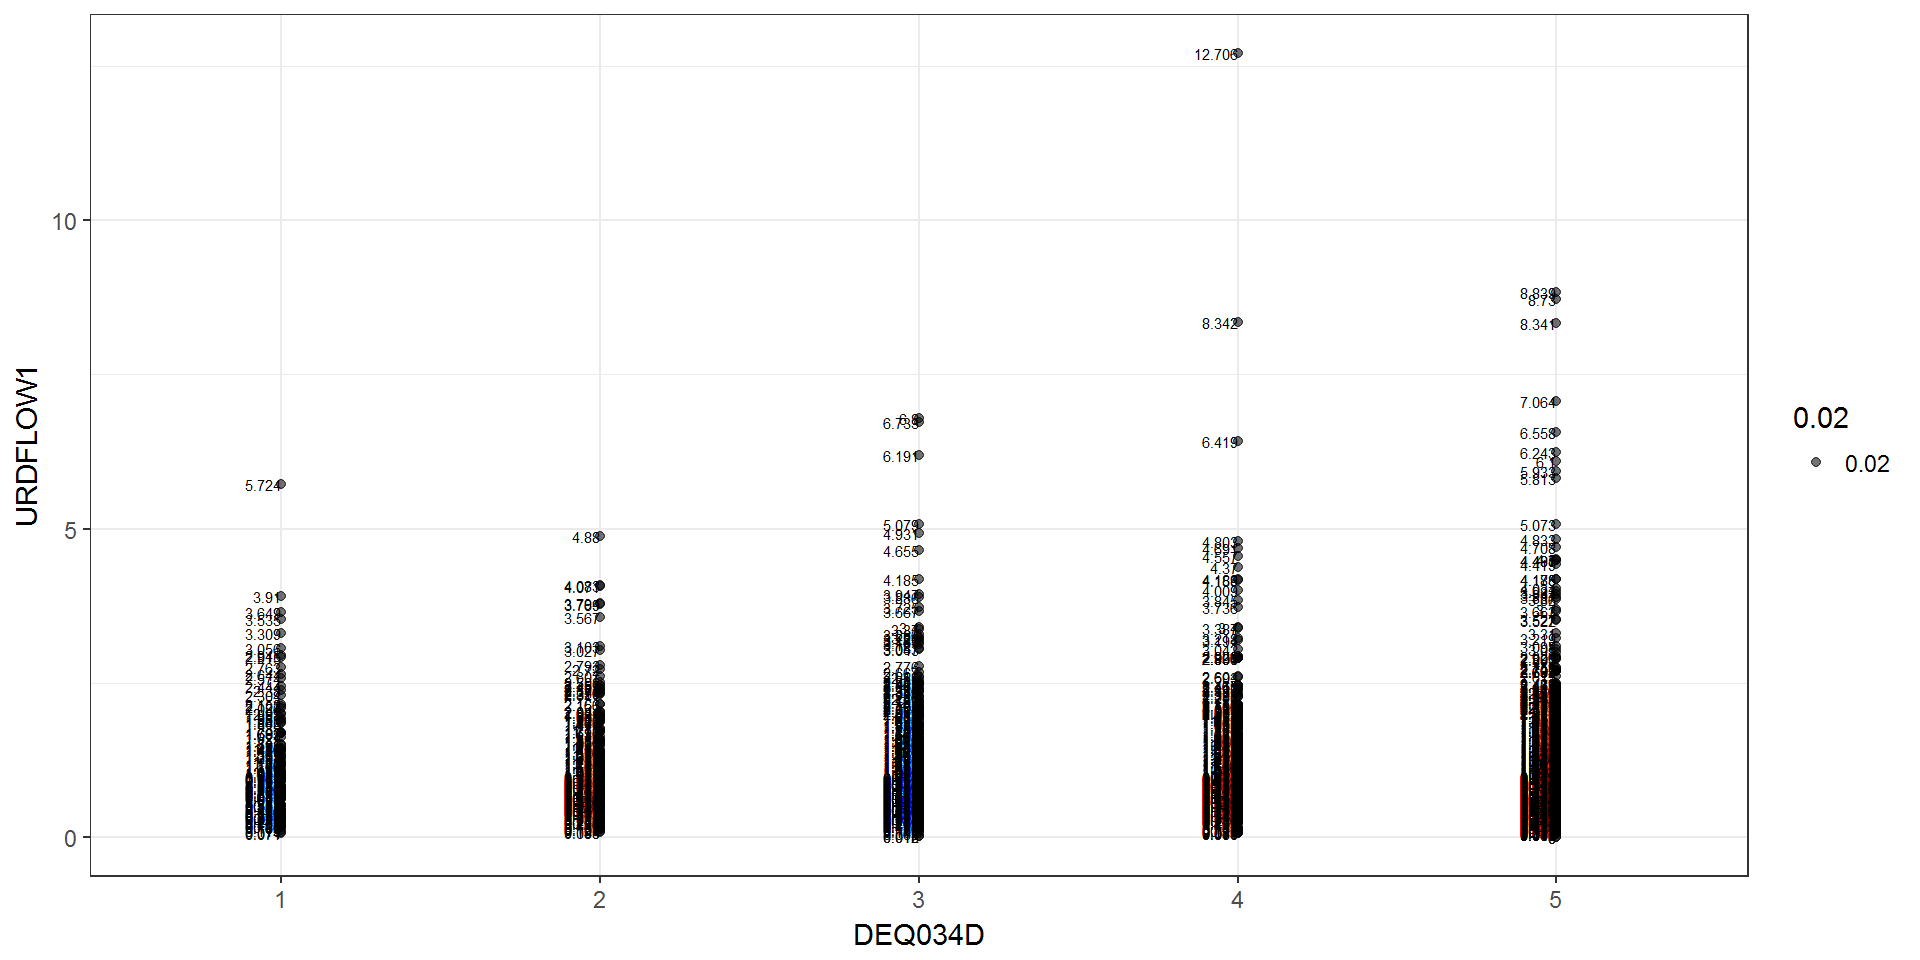
\includegraphics[width=5in]{graph.png} 
  \caption{Sunscreen Use and Urine Flow Rate Graph.}
  \label{fig:Graph_SD} 
\end{figure} 

From the above graph we can ascertain to a certain degree that as the value of sunscreen column increases the urine flow rate increases. From the above table we can rewrite it as the less a person applies sunscreen the more better his urine flow rate will be. However, this analysis needs to be taken with a pinch of salt. As stated before, due to null values several columns were omitted. Therefore, there may be a column which would better explain the confusing relationship shown above.
\vspace{5mm}The entire code for this study has been placed in the following GitHub location - \textbf{https://github.com/tanmayatripathi}

\section{Experimental Setup} \label{experiment}

For our study we used two machine learning algorithms, apart from Logistic Regression. They are Decision Trees and Random Forest. To start with we loaded the rpart and randomForest library into R to perform the ML operations. Since the size of our data set was small we did not limit the size of the trees. Hence, we developed the models with default conditions.
\vspace{5mm}For Random Forest we did provide the importance parameter as TRUE. This was to understand which variable was how important in determining the accuracy of the data. The result of the ML models is available in the later sections. The code executed has been placed at the following GitHub location - \textbf{https://github.com/tanmayatripathi}.

\subsection{Cohort Selection} 

For our study the cohort was selected from the NHANES population and consisted of men of age group 20-45. Due to the massive number of columns not all of them can be displayd in the demographics table below. However, we have tried to show a few of them.

\begin{table}[htbp]
  \centering 
  \begin{tabular}{lclc} 
    Column Name & Yes and No (\%) \\ 
    \hline \\[-11pt]
    Urine Flow Normal & Yes(1740[87.83\%]), No(241[12.17\%]) \\ 
    Health Insurance & Yes(1346[67.95\%]), No(635[32.05\%]) \\ \hline 
  \end{tabular}
  \label{tab:demogrpahics} 
    \caption{Cohort selection.} 
\end{table}

The data was then randomised and has been split into groups of two. One was the trial group and the other ended up as the test group.

\subsection{Data Extraction} 

Majority of the columns that were selected had complete data within them. The few that did not have were removed from the analysis. Unfortunately, this significantly reduced our sample size to 1,981 rows. Due to the nature of the data it was difficult to impute the column with self realized values. However, for the column ALQ101 we have imputed No for null values. By looking at the alcohol questuonairre dataset we realized that it is possible that the patient/physician did not mark the answer to the question since the patient said no.


\subsection{Feature Choices} 
The features were extracted from the NHANES data set. For our analysis we extracted Features from the demmographics, laboratory and questionairre sections. In majority of the cases we had sufficient data for demographics. Unfortunately, the data for urine labs was collected from 2009 onwards and therefore we had to limit ourselves to 2009 and beyond. The outcome variable URDFLOW1\_STATE was derived from the column URDFLOW1. A healthy urine flow rate is observerd in the range of 20mL/s or greater (a). Therefore, anything below the range was classified as abnormal while a healthy flow rate was classified as normal.

\url a. https://www.ncbi.nlm.nih.gov/pmc/articles/PMC1472847/

\subsection{Evaluation Criteria}
To evaluate the usefulness of the model, we implemented two evaluation techniques, one is the confusion matrix and the other one is the ROC curve. The confusion matrix is an important parameter because it shows how accurately the model predicted compared to the original values. The ROC curve highlights the accuracy of the model and shows the relation between the true positive rate and the false positive rate.

\section{Results} \label{results}

As described in the earlier sections we split our data into Train and Test set to run on the two ML algorithms. The models were developed using the train data set and were then compared with the test set. The split between the train and test were about 50\%.

\vspace{5mm} The confusion matrix of the two models has been shown in table 2.
\begin{table}[htbp]
  \centering 
  \begin{tabular}{lclc} 
    Model Name & Train Accuracy & Test Accuracy \\ 
    \hline \\[-11pt]
    Decision Tree & 88.38\% & 86.58\% \\ 
    Random Forest & 100\% & 86.89\% \\ \hline 
  \end{tabular}
  \label{tab:conf_matrix} 
    \caption{Confusion Matrix.} 
\end{table}

As we can see from the above result, Decision Tree on an average has given about 87\% accuracy which is close to the baseline. RandomForest on the other hand has a train accuracy of 100\% but drops down to decision tree accuracy level when test set is compared. This means that there is still an issue over fitting in the models which needs to be resolved.

\vspace{5mm} To further evaluate the models we plotted the ROC curves. For this exercise we took the entire data in the training set. Furthermore, we also included the Logistic Regression model for this analysis. The output of the ROC is shown in figure 4.

\begin{figure}[htbp]
  \centering 
  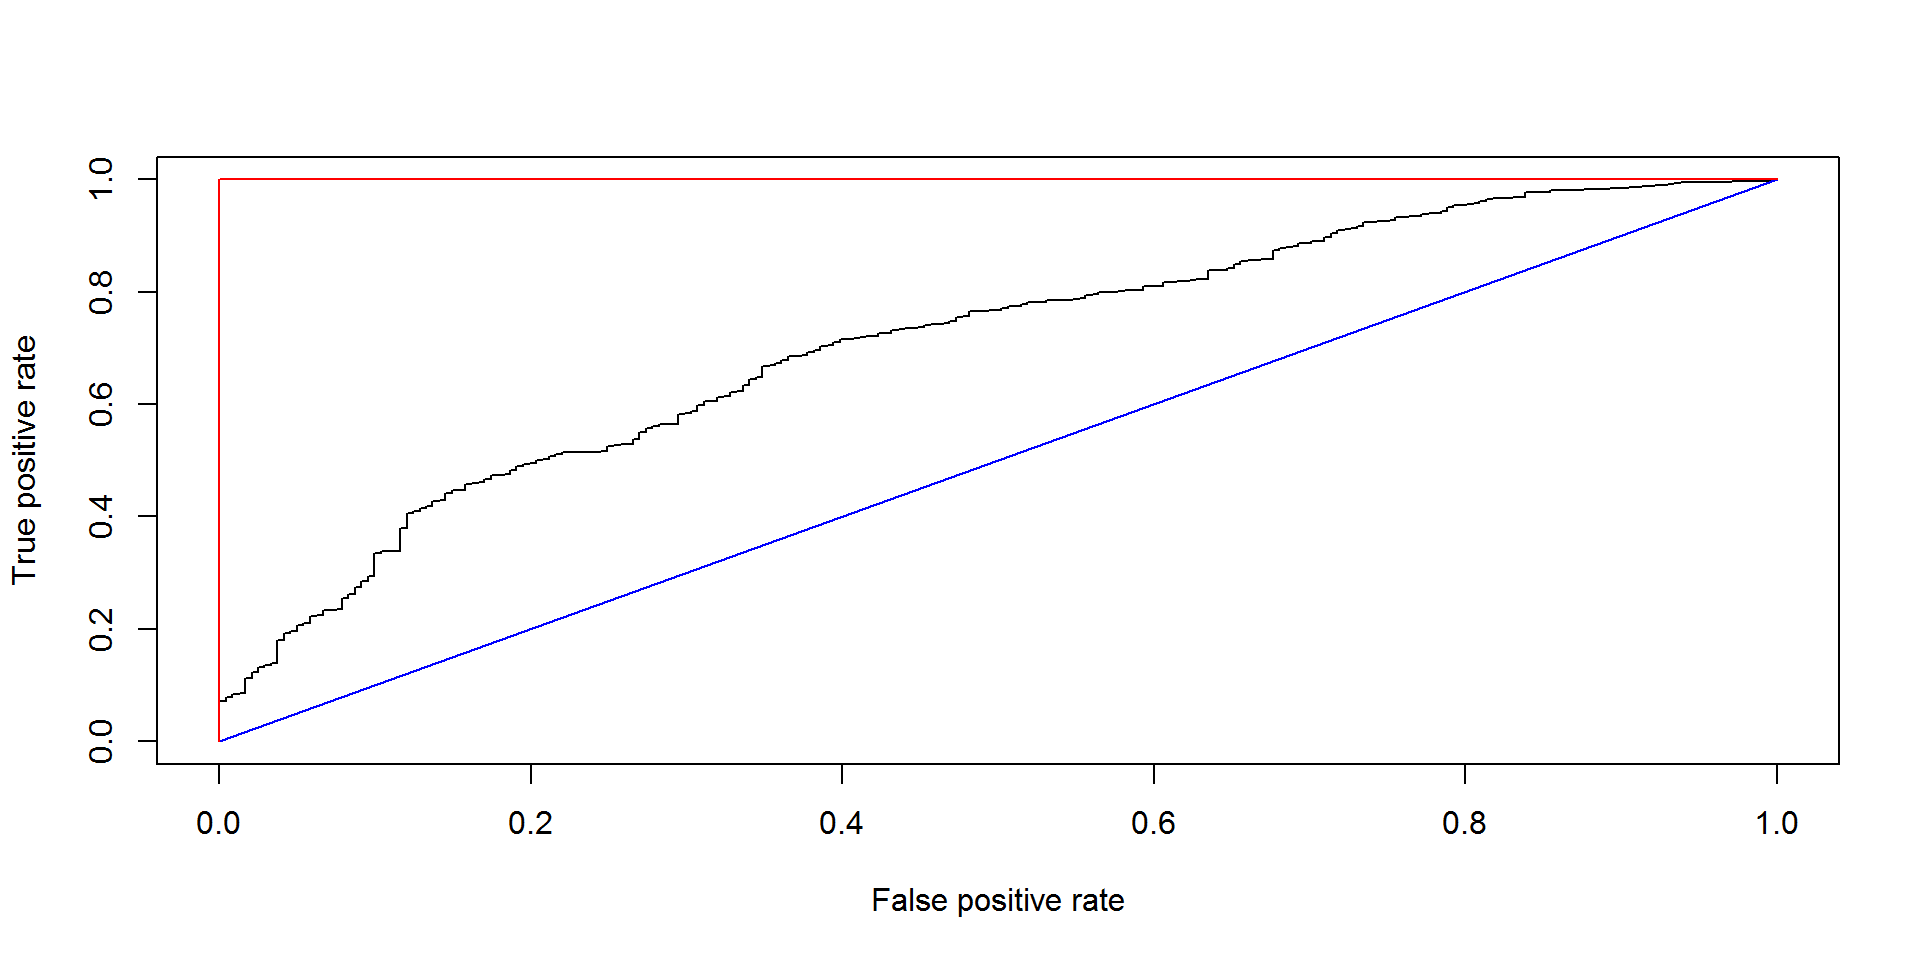
\includegraphics[width=5.5in]{roc_curve.png} 
  \caption{ROC Curve.}
  \label{fig:roc_curve} 
\end{figure} 

From the ROC curve we can see that randomForest (red) has a perfect curve while Decision Tree (blue) is near randomization. Logistic Regression is in the middle of the two (black).

\section{Discussion and Related Work} 

From the above outcomes we can see that it is possible to understand a patient's urine flow rate by his lifestyle choices. Therefore, the study shows NHANES data is a goldmine to conduct such kind of studies. Unfortunately, the NHANES data is not that robust. Although it has all the fields one would need in his/her study, the data is plagued with null values, incorrect data etc.

\vspace{5mm} The study was able to find only one significant field which is the correlation between use of sunscreen and urine flow rate. Unfortunately, given how many columns we had to omit due to null values, it is possible that there is a certain column which we left out, which would have done a much better job of explaining the relation. However, we can be sure to a certain extant that there is some type of relation. Whether that relation is indirect or direct needs to be looked into further.

\section{Conclusion} 
In conclusion, the NHANES data does contain certain columns that maybe used to describe the lifestyle changes of a patient and how it has affected the patient's health. However, the data filling guidelines need to be more rigorous to make the data more easy to interpret. As a next step to the study we are planning to look into the questionairre data further. We would also look into as to how the values are entered by the patient/physician. This would ultimately help us to impute the missing values and help build a much accurate model.

% ACKNOWLEDGEMENTS ONLY GO IN THE CAMERA-READY, NOT THE SUBMISSION
% \acks{Many thanks to all collaborators and funders!}

\appendix
\section*{Appendix A.}
\textbf{Code available at the following repository - }https://github.com/tanmayatripathi

\end{document}
